
\section{\texorpdfstring{$L$}{L} 的\trIndex{}的计算}
\label{sec:index-computation}

为了计算 $L$ 的\trIndex，
\[
L(Y)=\frac{\partial Y}{\partial s}+J_0\frac{\partial Y}{\partial t}+S(s,t)Y\text{，}
\]
其中 $\lim_{s\to\pm\infty}S(s,t)=S^{\pm}(t)$（对 $t$ \trUniform），我们将要：
\begin{enumerate}[label=(\arabic*)]
\item 把 $L$ 换成 $L_0$，后者由同一个公式给出……只不过 $S(s,t)$ 换成了一个矩阵 $\widetilde{S}(s,t)$，它在 $s\le-\sigma_0$ 时\emph{恰好}是 $S^{-}(t)$，在 $s\ge\sigma_0$ 时\emph{恰好}是 $S^{+}(t)$。\trIndex{}在小\trPerturbation{}下的不变性（当 $\sigma_0$ 充分大时）将蕴含 $L_0$ 的\trIndex{}与 $L$ 的相同。这就是\cref{thm:index-plateau}。
\item 再把 $L_0$ 换成 $L_1$，后者仍由同一个公式给出，但其中 $\widetilde{S}(s,t)$ 换成了一个\emph{对角}矩阵 $S(s)$（它不依赖于 $t$），并且它在 $s\le-\sigma_0$ 与 $s\ge\sigma_0$ 时为常值。这一次，$L_1$ 将与 $L_0$ 具有相同的\trIndex，其依据是\trIndex{}在\trHomotopy{}下的不变性（以及极限对角矩阵的构造）。这就是\cref{thm:index-diagonal-perturbation}与\cref{thm:index-k-minus}。
\end{enumerate}

这一过程概述于\cref{fig:matrices-cylinders}之中，图中在矩阵空间里表示了出现于算子 $L$、$L_0$ 与 $L_1$ 中的那些不同的映射 $S(s,t)$：外面的“圆柱”是 $S(s,t)$（原来的那一个），粗圆柱是 $\widetilde{S}(s,t)$（我们在无穷远处把 $S$ 逼近成了真正的圆柱），而由对角矩阵构成的那条虚线则表示矩阵 $S(s)$（即 $L_1$ 的那一个）。

\begin{figure}[htbp]
\centering
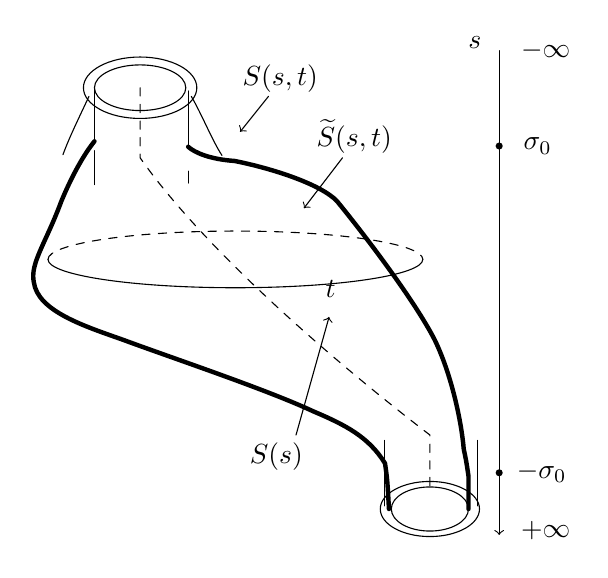
\begin{tikzpicture}[scale=1.0,line cap=round,line join=round]
  \draw (1.2,2.53) ellipse (0.72 and 0.39);
  \draw (1.2,2.53) ellipse (0.58 and 0.29);
  \draw (0.62,2.53) -- (0.62,1.85);%
  \draw (1.81,2.49) -- (1.81,1.78);%
  \draw (0.55,2.42) .. controls (0.42,2.14) and (0.3,1.9) .. (0.22,1.68);%
  \draw (1.85,2.42) .. controls (1.98,2.2) and (2.12,1.85) .. (2.24,1.67);%
  \draw (0.62,1.73) -- (0.62,1.30);%
  \draw (1.82,1.47) -- (1.82,1.32);%
  \draw[line width=1.6pt] (0.62,1.85)
        .. controls (0.5,1.7) and (0.35,1.45) .. (0.2,1.09)
        .. controls (0.0,0.55) and (-0.2,0.3) .. (-0.15,0.06)
        .. controls (-0.1,-0.31) and (0.5,-0.5) .. (0.98,-0.67)
        .. controls (1.6,-0.9) and (2.8,-1.3) .. (3.4,-1.58)
        .. controls (3.8,-1.75) and (4.1,-1.9) .. (4.31,-2.24)
        .. controls (4.34,-2.45) .. (4.36,-2.82);
  \draw[line width=1.6pt] (1.81,1.78)
        .. controls (1.9,1.7) and (2.1,1.62) .. (2.4,1.6)
        .. controls (2.9,1.5) and (3.5,1.3) .. (3.7,1.09)
        .. controls (4.1,0.6) and (4.7,-0.2) .. (4.94,-0.67)
        .. controls (5.15,-1.1) and (5.28,-1.7) .. (5.31,-2.06)
        .. controls (5.34,-2.2) .. (5.37,-2.4)
        -- (5.37,-2.82);
  \draw (4.88,-2.82) ellipse (0.63 and 0.35);
  \draw (4.88,-2.82) ellipse (0.49 and 0.28);
  \draw (4.30,-1.95) -- (4.30,-2.78);%
  \draw (5.49,-1.95) -- (5.49,-2.78);%
  \draw[dashed] (1.2,2.53) -- (1.2,1.64)
        .. controls (2.0,0.5) and (3.6,-0.9) .. (4.88,-1.88)
        -- (4.88,-2.62);
  \draw (0.03,0.35) arc (180:360:2.38 and 0.36);
  \draw[dashed] (0.03,0.35) arc (180:0:2.38 and 0.36);
  \node at (3.62,-0.02) {$t$};
  \node at (2.98,2.64) {$S(s,t)$};
  \draw[->] (2.83,2.42) -- (2.47,1.97);
  \node at (3.92,1.91) {$\widetilde{S}(s,t)$};
  \draw[->] (3.77,1.64) -- (3.28,1.0);
  \node at (2.93,-2.15) {$S(s)$};
  \draw[->] (3.18,-1.88) -- (3.6,-0.38);
  \draw[->] (5.76,3.0) -- (5.76,-3.15);
  \node at (5.45,3.1) {$s$};
  \node at (6.35,3.0) {$-\infty$};
  \fill (5.76,1.79) circle (0.045);
  \node at (6.25,1.79) {$\sigma_0$};
  \fill (5.76,-2.36) circle (0.045);
  \node at (6.3,-2.36) {$-\sigma_0$};
  \node at (6.35,-3.1) {$+\infty$};
\end{tikzpicture}
\caption{}
\label{fig:matrices-cylinders}
\end{figure}

\subsection{\trFredholm{}\trIndex}
\label{subsec:fredholm-index}

我们考虑算子
\[
\begin{array}{c}
L\colon W^{1,p}(\RR\times S^{1};\RR^{2n})\longrightarrow L^{p}(\RR\times S^{1};\RR^{2n})\\[4pt]
Y\longmapsto\dfrac{\partial Y}{\partial s}+J_0\dfrac{\partial Y}{\partial t}+S(s,t)Y\text{。}
\end{array}
\]
回想一下，$S\colon\RR\times S^{1}\to M(2n;\RR)$ 满足
\[
\lim_{s\to\pm\infty}S(s,t)=S^{\pm}(t)\quad\text{（对 $t$ \trUniform）}
\]
其中诸 $S^{\pm}(t)$（对每个 $t\in S^{1}$）都是\trSymmetricMatrix。考虑与这两个矩阵 $S^{\pm}$ 相伴的\trSymplectic{}道路（参见\cref{subsec:symplectic-symmetric-link}）
\[
R^{\pm}\colon[0,1]\longrightarrow\mathrm{Sp}(2n;\RR)\text{。}
\]
\cref{thm:hamiltonian-linearization}表明，这些道路恰好就是定义（\trConleyZehnderIndex）$\mu(x)$ 与 $\mu(y)$ 的那些道路。我们已经证明过（\cref{thm:fredholm-operator-L}），若 $R^{\pm}$ 属于那些满足 $R(0)=\mathrm{Id}$ 且 $\det(R(1)-\mathrm{Id})\ne 0$ 的道路 $R(t)$ 所成的集合 $\scr{S}$，则 $L$ 是一个\trFredholmOperator。我们现在就来计算它的\trIndex。

\begin{theorem}\label{thm:index-maslov-difference}
\trFredholmOperator{} $L$ 的\trIndex{}为
\[
\mu(R^{-}(t))-\mu(R^{+}(t))=\mu(x)-\mu(y)\text{。}
\]
\end{theorem}

令 $k^{\pm}$ 表示 $R^{\pm}(t)$ 的\trIndex。我们要用到\cref{subsec:prescribed-maslov-index}的记号，特别是\cref{thm:prescribed-maslov-index}所给出的那些矩阵 $S_{k\pm}$。本定理将是下面两条命题的推论。

\begin{proposition}\label{thm:index-diagonal-perturbation}
设 $s_0$ 是一个正实数，并设
\[
S\colon\RR\longrightarrow M(2n;\RR)
\]
是一条由对角矩阵构成的道路，它在 $s\le-s_0$ 时 $S(s)=S_{k-}$，在 $s\ge s_0$ 时 $S(s)=S_{k+}$。令
\[
\begin{array}{c}
L_1\colon W^{1,p}(\RR\times S^{1};\RR^{2n})\longrightarrow L^{p}(\RR\times S^{1};\RR^{2n})\\[4pt]
Y\longmapsto\dfrac{\partial Y}{\partial s}+J_0\dfrac{\partial Y}{\partial t}+S(s)Y\text{。}
\end{array}
\]
那么，\trFredholmOperator{} $L_1$ 的\trIndex{}与 $L$ 的相同。
\end{proposition}

\begin{proposition}\label{thm:index-k-minus}
$L_1$ 的\trIndex{}为 $k^{-}-k^{+}$。
\end{proposition}

为了证明\cref{thm:index-diagonal-perturbation}，我们将在\trFredholmOperator{}的集合内部修改 $L$ 而不改变它的\trIndex。

\begin{lemma}\label{thm:index-plateau}
$L$ 的\trIndex{}与算子 $L_0$ 的\trIndex{}相同，在 $L_0$ 中，$S(s,t)$ 在 $s\le-s_0$ 时被换成 $S^{-}(t)$，在 $s\ge s_0$ 时被换成 $S^{+}(t)$。
\end{lemma}

\begin{proof}
我们取定一个实数 $\varepsilon>0$。由于矩阵 $S(s,t)$ 在 $s\to\pm\infty$ 时趋于 $S^{\pm}(t)$，故存在一个实数 $\sigma_0$，使得
\[
\left\{\begin{array}{ll}
\text{对 }s\le-\sigma_0\text{，} & \|S(s,t)-S^{-}(t)\|<\varepsilon\text{，}\\
\text{对 }s\ge\sigma_0\text{，} & \|S(s,t)-S^{+}(t)\|<\varepsilon\text{。}
\end{array}\right.
\]
我们考虑一个\trPlateauFunction{} $\chi\colon\RR\to[0,1]$，它在 $|s|\le\sigma_0$ 时取值 $1$，在 $|s|\ge 2\sigma_0$ 时取值 $0$。令
\[
\Sigma(s,t)=\left\{\begin{array}{ll}
\chi(s)S(s,t)+(1-\chi(s))S^{-}(t) & \text{若 }s\le-\sigma_0\\
S(s,t) & \text{若 }|s|\le\sigma_0\\
\chi(s)S(s,t)+(1-\chi(s))S^{+}(t) & \text{若 }s\ge\sigma_0\text{，}
\end{array}\right.
\]
并让 $L_0$ 定义为
\[
L_0(Y)=\frac{\partial Y}{\partial s}+J_0\frac{\partial Y}{\partial t}+\Sigma Y\text{。}
\]
于是 $LY=L_0Y+C(s,t)Y$，其中
\[
C(s,t)=\left\{\begin{array}{ll}
(1-\chi(s))(S(s,t)-S^{-}(t)) & \text{若 }s\le-\sigma_0\\
0 & \text{若 }|s|\le\sigma_0\\
(1-\chi(s))(S(s,t)-S^{+}(t)) & \text{若 }s\ge\sigma_0\text{。}
\end{array}\right.
\]
特别地，$\|C(s,t)\|<\varepsilon$。若 $\varepsilon$ 充分小，那么我们知道（这就是\trIndex{}在小\trPerturbation{}下的不变性，即\cref{thm:appC-index-stability}）：$L_0$ 是一个\trFredholmOperator，并且它与 $L$ 具有相同的\trIndex。

现在，$\Sigma(s,t)$ 在 $|s|\ge 2\sigma_0$ 时与 $S^{\pm}(t)$ 重合，而我们想要的却是把这条性质中的 $\sigma_0$ 换成 $s_0$（$\sigma_0$ 是由 $\varepsilon$ 的选取确定的）。只需用一条在 $s$ 充分大时为常值的道路，把 $\Sigma(s,t)$ 连接到以同样方式如下定义的
\[
\Sigma_0(s,t)=\left\{\begin{array}{ll}
S^{-}(t) & \text{若 }s\le-s_0\\
S^{+}(t) & \text{若 }s\ge s_0\text{，}
\end{array}\right.
\]
即可。由这条道路所定义的那些算子的\trFredholm{}\trIndex{}为常数，这由局部常值性这一同样的性质得到（参见\cref{thm:appC-index-continuity}）。
\end{proof}

我们将会用到\cref{subsec:symplectic-symmetric-link}中所建立的、$\mathrm{Sp}(2n)$ 中的道路与方程
\[
\frac{dY}{dt}=J_0S(t)Y
\]
之解的基本矩阵 $R(t)$ 之间的联系——这些方程我们已经在\cref{thm:a-invertible-p2}的证明中考虑过了——以及\cref{subsec:prescribed-maslov-index}中构造的具有指定\trMaslovIndex{}的道路。

\begin{proof}[\cref{thm:index-diagonal-perturbation}的证明]
\cref{thm:prescribed-maslov-index}的证明中的那些对角矩阵 $S_k$ 定义了\trSymplectic{}道路 $R_{k\pm}(t)=e^{tJ_0S_{k\pm}}$，\footnote{译注：原书此处印作 $e^{tJS_{k\pm}}$，$J$ 无下标；按\cref{thm:symplectic-symmetric-paths}与\cref{thm:prescribed-maslov-index}的记号应作 $J_0$（下文 $S_\lambda^{\pm}$ 一式同），此处径改。——译者注}它们的\trMaslovIndex{}（即 $k^{\pm}$）与 $R^{\pm}(t)$ 的相同。于是存在（由\cref{thm:sp-star-components}）一个\trHomotopy{} $\psi^{\pm}(\lambda,t)$，
\[
\psi^{\pm}\colon[0,1]\times[0,1]\longrightarrow\mathrm{Sp}(2n)
\]
（对每个 $\lambda$ 都有 $\psi^{\pm}(\lambda,\cdot)\in\scr{S}$），它连接 $R_{k\pm}(t)$ 与 $R^{\pm}(t)$，我们可以、而且也确实假设它是 $\cC^{1}$ 类的。正如我们在\cref{thm:symplectic-symmetric-paths}中已经指出过的那样，这条\trSymplectic{}矩阵的道路生成一条由\trSymmetricMatrix{}构成的道路
\[
S_\lambda^{\pm}(t)=-J_0\dot{\psi}_\lambda^{\pm}(t)\bigl(\psi_\lambda^{\pm}(t)\bigr)^{-1}\text{。}
\]
唯一的问题在于，我们的变量 $t$ 取值于 $S^{1}$ 中；因此我们想要关于 $t$ \trPeriodic{}的道路。为了做到这一点，我们如下修改这些\trHomotopy{} $\psi^{\pm}$。我们用一个递增的 $\cC^\infty$ 函数
\[
\chi\colon[0,1]\longrightarrow[0,1]
\]
它在 $0$ 附近取值 $0$，在 $1$ 附近取值 $1$，以及一个连接 $\chi$ 与 $\mathrm{Id}$ 的\trHomotopy{} $\chi_\lambda$。与 $R_{k\pm}(\chi_\lambda(t))$ 相伴的\trSymmetricMatrix{}道路是 $\dot{\chi}_\lambda(t)S_{k\pm}$；如果我们这样选取\trHomotopy{}使得 $\dot{\chi}_\lambda(0)=\dot{\chi}_\lambda(1)$，那么它就是\trPeriodic{}的。同样地，我们用\trHomotopy{} $R(\chi_\lambda(t))$ 连接道路 $R^{\pm}(t)$ 与 $R^{\pm}(\chi(t))$，其相伴的那些\trSymmetricMatrix{}道路对每个 $\lambda$ 都是\trPeriodic{}的。然后我们考虑\trHomotopy{} $\psi^{\pm}(\lambda,\chi(t))$。其相伴的那些\trSymmetricMatrix{}道路在 $t=0$ 与 $t=1$ 附近为零，从而特别地是\trPeriodic{}的。\footnote{译注：原书自上一式起把\trHomotopy{} $\psi^{\pm}(\lambda,t)$ 及其相伴的对称道路缩写作 $\psi_\lambda^{\pm}(t)$ 与 $S_\lambda^{\pm}(t)$（$\lambda$ 固定）。——译者注}

我们由此得到了映射
\[
S^{\pm}\colon[0,1]\times S^{1}\longrightarrow M(2n;\RR)
\]
它取值于\trSymmetricMatrix{}的空间中，使得对每个 $\lambda\in[0,1]$，$t\mapsto S^{\pm}(\lambda,t)$ 都生成 $\scr{S}$ 中的一条道路，并且我们有：
\begin{itemize}
\item $S^{\pm}(0,t)$ 生成 $R^{\pm}(t)$。
\item $S^{\pm}(1,t)=S_{k\pm}$ 不依赖于 $t$，生成 $R_{k\pm}(t)$。
\end{itemize}
然后我们就能定义一个连续映射
\[
S\colon[0,1]\times\RR\times S^{1}\longrightarrow M(2n;\RR)
\]
使得
\[
S_\lambda(s,t)=\left\{\begin{array}{ll}
S(s,t) & \text{若 }\lambda=0\\
S_\lambda^{+}(t) & \text{若 }s\ge\sigma_0\\
S_\lambda^{-}(t) & \text{若 }s\le-\sigma_0\\
S(s) & \text{若 }\lambda=1\text{。}
\end{array}\right.
\]
这就定义了一族算子
\[
\begin{array}{c}
L_\lambda\colon W^{1,p}(\RR\times S^{1};\RR^{2n})\longrightarrow L^{p}(\RR\times S^{1};\RR^{2n})\\[4pt]
Y\longmapsto\dfrac{\partial Y}{\partial s}+J_0\dfrac{\partial Y}{\partial t}+S_\lambda(s,t)Y\text{，}
\end{array}
\]
它们都是\trFredholmOperator（仍由\cref{thm:fredholm-operator-L}），并且都具有相同的\trIndex（由不变性\cref{thm:appC-index-stability}）。算子 $L_1$ 就是该命题中所宣布的那一个。
\end{proof}

\begin{proof}[\cref{thm:index-k-minus}的证明]
在\cref{thm:fredholm-operator-L}的证明中，我们用到过 $\operatorname{Coker}L_1$ 与 $\operatorname{Ker}L_1^{\star}$ \trIsomorphic{}这一事实，其中 $L_1$ 的\trAdjointOperator{} $L_1^{\star}$ 为
\[
\begin{array}{c}
L_1^{\star}\colon W^{1,q}(\RR\times S^{1};\RR^{2n})\longrightarrow L^{q}(\RR\times S^{1};\RR^{2n})\\[4pt]
Z\longmapsto-\dfrac{\partial Z}{\partial s}+J_0\dfrac{\partial Z}{\partial t}+{}^{t}S(s)Z\text{，}
\end{array}
\]
其中 $1/p+1/q=1$。因此，只需对这一类型的算子计算其\trKernel{}的维数。由于
\[
J_0=\left(\begin{array}{cccc}
\left(\begin{array}{cc}0&-1\\1&0\end{array}\right)&&&\\
&\ddots&&\\
&&&\left(\begin{array}{cc}0&-1\\1&0\end{array}\right)
\end{array}\right)
\]
属于 $M(2;\RR)\times\cdots\times M(2;\RR)$，我们可以化归到 $n=1$ 的情形。于是我们假设对角矩阵 $S(s)$ 是形如
\[
S(s)=\left(\begin{array}{cc}
a_1(s) & 0\\
0 & a_2(s)
\end{array}\right)\text{，}\qquad
\text{其中 }a_i(s)=\left\{\begin{array}{ll}
a_i^{-} & \text{若 }s\le-s_0\text{，}\\
a_i^{+} & \text{若 }s\ge s_0
\end{array}\right.
\]
的 $2\times 2$ 矩阵。我们现在证明下面这个结果。

\begin{lemma}\label{thm:kernel-dimension-diagonal}
设 $p>2$，并设
\[
F\colon W^{1,p}(\RR\times S^{1};\RR^{2})\longrightarrow L^{p}(\RR\times S^{1};\RR^{2})
\]
由
\[
F(Y)=\frac{\partial Y}{\partial s}+J_0\frac{\partial Y}{\partial t}+S(s)Y
\]
定义。我们假设 $a_i^{\pm}\notin 2\pi\ZZ$：
\begin{enumerate}[label=(\arabic*)]
\item 设 $a_1(s)=a_2(s)$。记 $a^{\pm}=a_1^{\pm}=a_2^{\pm}$。那么
\[
\begin{array}{l}
\dim\operatorname{Ker}F=2\,\#\bigl\{\ell\in\ZZ\ \big|\ a^{-}<2\pi\ell<a^{+}\bigr\}\\[2pt]
\dim\operatorname{Ker}F^{\star}=2\,\#\bigl\{\ell\in\ZZ\ \big|\ a^{+}<2\pi\ell<a^{-}\bigr\}
\end{array}
\]
\item 设 $\sup_{s\in\RR}\|S(s)\|<1$。那么
\[
\begin{array}{l}
\dim\operatorname{Ker}F=\#\bigl\{i\in\{1,2\}\ \big|\ a_i^{-}<0\ \text{且}\ a_i^{+}>0\bigr\}\\[2pt]
\dim\operatorname{Ker}F^{\star}=\#\bigl\{i\in\{1,2\}\ \big|\ a_i^{+}<0\ \text{且}\ a_i^{-}>0\bigr\}\text{。}
\end{array}
\]
\end{enumerate}
\end{lemma}

\begin{remark}\label{thm:morse-index-formula}
这与在\trMorse{}情形中借助变号\trEigenvalue{}的个数来计算\trIndex{}的那条公式相当接近（参见关于命题~10.2.8 之证明的注记）。
\end{remark}

\cref{thm:kernel-dimension-diagonal}的证明是对\trKernel{}的一个显式计算，我们稍后再给出它。现在来看看，如果我们暂时承认这条引理，该如何利用它来计算 $L_1$ 的\trIndex{}，从而完成\cref{thm:index-k-minus}的证明。按照 $k^{+}-n$ 与 $k^{-}-n$ 的可能奇偶性，我们需要区分四种情形。

\begin{enumerate}[label=(\arabic*)]
\item 情形 $S_{k-}$ 与 $S_{k+}$ 为对角矩阵
\[
\left\{\begin{array}{l}
S_{k-}=(-\pi,-\pi,\dotsc,-\pi,-\pi,(n-1-k^{-})\pi,(n-1-k^{-})\pi)\\
S_{k+}=(-\pi,-\pi,\dotsc,-\pi,-\pi,(n-1-k^{+})\pi,(n-1-k^{+})\pi)\text{，}
\end{array}\right.
\]
其中 $k^{-}\equiv k^{+}\equiv n\ \mathrm{mod}\ 2$。我们可以取 $a_1(s)=a_2(s)$，于是 $a_1^{\pm}=a_2^{\pm}$，而\cref{thm:kernel-dimension-diagonal}给出
\[
\begin{aligned}
\dim\operatorname{Ker}L_1
&=2\,\#\bigl\{\ell\in\ZZ\mid n-1-k^{-}<2\ell<n-1-k^{+}\bigr\}\\
&=\left\{\begin{array}{ll}
k^{-}-k^{+} & \text{若 }k^{-}>k^{+}\text{，}\\
0 & \text{否则，}
\end{array}\right.
\end{aligned}
\]
而
\[
\begin{aligned}
\dim\operatorname{Ker}L_1^{\star}
&=2\,\#\bigl\{\ell\in\ZZ\mid k^{-}-n+1<2\ell<k^{+}-n+1\bigr\}\\
&=\left\{\begin{array}{ll}
k^{+}-k^{-} & \text{若 }k^{+}>k^{-}\text{，}\\
0 & \text{否则。}
\end{array}\right.
\end{aligned}
\]
因此，
\[
\operatorname{Ind}(L_1)=k^{-}-k^{+}\text{。}
\]
\item 情形 $S_{k-}$ 与 $S_{k+}$ 为对角矩阵
\[
\left\{\begin{array}{l}
S_{k-}=(-\pi,-\pi,\dotsc,-\varepsilon\pi,-\varepsilon\pi,(n-1-k^{-})\pi,(n-1-k^{-})\pi)\\
S_{k+}=(-\pi,-\pi,\dotsc,\varepsilon,-\varepsilon,(n-2-k^{+})\pi,(n-2-k^{+})\pi)\text{，}
\end{array}\right.
\]
其中 $k^{-}\equiv n\ \mathrm{mod}\ 2$ 而 $k^{+}\equiv n-1\ \mathrm{mod}\ 2$。在这个情形中，我们取 $a_1(s)=a_2(s)$，但第 $(n-1)$ 个分块除外，对这个分块我们可以假设 $\sup_{s\in\RR}\|S(s)\|<1$。我们得到
\[
\begin{aligned}
\dim\operatorname{Ker}L_1
&=2\,\#\bigl\{\ell\in\ZZ\mid n-1-k^{-}<2\ell<n-2-k^{+}\bigr\}+1\\
&=\left\{\begin{array}{ll}
(k^{-}-k^{+}-1)+1 & \text{若 }k^{-}>k^{+}\text{，}\\
1 & \text{若 }k^{-}<k^{+}\text{，}
\end{array}\right.
\end{aligned}
\]
而
\[
\begin{aligned}
\dim\operatorname{Ker}L_1^{\star}
&=2\,\#\bigl\{\ell\in\ZZ\mid k^{-}-n+1<2\ell<k^{+}-n+2\bigr\}\\
&=\left\{\begin{array}{ll}
k^{+}-k^{-}+1 & \text{若 }k^{+}>k^{-}\text{，}\\
0 & \text{否则。}
\end{array}\right.
\end{aligned}
\]
因此，在这个情形中我们同样有
\[
\operatorname{Ind}(L_1)=k^{-}-k^{+}\text{。}
\]
\item 情形 $S_{k-}$ 与 $S_{k+}$ 为对角矩阵
\[
\left\{\begin{array}{l}
S_{k-}=(-\pi,-\pi,\dotsc,\varepsilon,-\varepsilon,(n-2-k^{-})\pi,(n-2-k^{-})\pi)\\
S_{k+}=(-\pi,-\pi,\dotsc,-\varepsilon\pi,-\varepsilon\pi,(n-1-k^{+})\pi,(n-1-k^{+})\pi)\text{，}
\end{array}\right.
\]
这一次是 $k^{-}\equiv n-1\ \mathrm{mod}\ 2$ 而 $k^{+}\equiv n\ \mathrm{mod}\ 2$。在这个情形中，我们同样有（把 $S_{k-}$ 与 $S_{k+}$ 的角色对调）
\[
\dim\operatorname{Ker}L_1=\left\{\begin{array}{ll}
k^{-}-k^{+}+1 & \text{若 }k^{-}>k^{+}\text{，}\\
0 & \text{否则，}
\end{array}\right.
\]
而
\[
\dim\operatorname{Ker}L_1^{\star}=\left\{\begin{array}{ll}
k^{+}-k^{-} & \text{若 }k^{+}>k^{-}\text{，}\\
1 & \text{否则，}
\end{array}\right.
\]
于是在这个情形中我们同样有
\[
\operatorname{Ind}(L_1)=k^{-}-k^{+}\text{。}
\]
\item 这就只剩下 $S_{k-}$ 与 $S_{k+}$ 为对角矩阵
\[
\left\{\begin{array}{l}
S_{k-}=(-\pi,-\pi,\dotsc,1,-1,(n-2-k^{-})\pi,(n-2-k^{-})\pi)\\
S_{k+}=(-\pi,-\pi,\dotsc,1,-1,(n-2-k^{+})\pi,(n-2-k^{+})\pi)\text{，}
\end{array}\right.
\]
且 $k^{+}\equiv k^{-}\equiv n-1\ \mathrm{mod}\ 2$ 的情形。我们有（对 $a_1(s)=a_2(s)$）
\[
\dim\operatorname{Ker}L_1=\left\{\begin{array}{ll}
k^{-}-k^{+} & \text{若 }k^{-}>k^{+}\text{，}\\
0 & \text{否则，}
\end{array}\right.
\]
而\footnote{译注：原书此式条件印作“$k^{-}>k^{+}$”（上一式则印作“$k^{+}>k^{-}$”）——按取值 $k^{+}-k^{-}$、$k^{-}-k^{+}$ 的符号，并与情形 (1) 的同款公式相对照，两条条件疑互换了位置，此处径改。——译者注}
\[
\dim\operatorname{Ker}L_1^{\star}=\left\{\begin{array}{ll}
k^{+}-k^{-} & \text{若 }k^{+}>k^{-}\text{，}\\
0 & \text{否则，}
\end{array}\right.
\]
并且，如同在其他情形中一样，我们仍有
\[
\operatorname{Ind}(L_1)=k^{-}-k^{+}\text{，}
\]
这就完成了\cref{thm:index-k-minus}的证明。
\end{enumerate}
\end{proof}

\begin{proof}[\cref{thm:kernel-dimension-diagonal}的证明]
我们从断言 (1) 开始。

记 $a(s)=a_1(s)=a_2(s)$。令
\[
\begin{aligned}
Y(s,t)&=(Y_1(s,t),Y_2(s,t))\in\RR^{2}\\
&=Y_1(s+it)+iY_2(s+it)\in\CC\text{。}
\end{aligned}
\]
偏\trDifferential{}方程 $F(Y)=0$ 可以写成
\[
\frac{\partial}{\partial s}\left(\begin{array}{c}Y_1\\Y_2\end{array}\right)
+\left(\begin{array}{cc}0&-1\\1&0\end{array}\right)\frac{\partial}{\partial t}\left(\begin{array}{c}Y_1\\Y_2\end{array}\right)
+\left(\begin{array}{cc}a(s)&0\\0&a(s)\end{array}\right)\left(\begin{array}{c}Y_1\\Y_2\end{array}\right)=0\text{，}
\]
亦即
\[
\bar{\partial}Y+S(s)Y=0\text{。}
\]
把未知函数换成 $Y=B\widetilde{Y}$，其中 $B$ 是一个复\trInvertible{}矩阵，满足
\[
\bar{\partial}B+SB=0\text{，}
\]
这就把这个方程变成了
\[
\bar{\partial}\widetilde{Y}=0
\]
（我们正在把这个方程变成\trCauchyRiemann{}方程，完全如同我们在\cref{sec:somewhere-injective}中所做的那样）。

最简单的解法是取 $B$ 为矩阵（属于 $\mathrm{GL}(1;\CC)\subset\mathrm{GL}(2;\RR)$）
\[
B=\left(\begin{array}{cc}
b(s) & 0\\
0 & b(s)
\end{array}\right)\qquad\text{其中 }b'=-ab\text{，}
\]
也就是说
\[
b(s)=\exp\int_0^{s}-a(\sigma)\,d\sigma=\exp(-A(s))\text{，}
\]
这正是我们此处所做的事情。我们不应忘记指出：在 $s\le-\sigma_0$ 时，$A(s)=C_1+a^{-}s$，同样地，在 $s\ge\sigma_0$ 时，$A(s)=C_2+a^{+}s$，其中 $C_1$ 与 $C_2$ 是某些常数。

新的未知函数 $\widetilde{Y}$ 满足\trCauchyRiemann{}方程 $\bar{\partial}\widetilde{Y}=0$。它是连续的、$L^{1}_{\mathrm{loc}}$ 的，因而由于\trEllipticRegularity（定理~12.1.3），它是\trSmooth{}的。它的实部与虚部 $\widetilde{Y}_1$ 与 $\widetilde{Y}_2$ 都是 $\cC^{\infty}$ 类的\trHarmonic{}函数。

现在我们把 $s+it\in\RR\times S^{1}$ 等同于 $u=e^{2\pi z}$，于是\trLaurent{}定理（对于 $\CC-\{0\}$ 上的 $\widetilde{Y}(u)$）便给出 $\widetilde{Y}$ 的展开。我们这个方程组的解因而是
\[
\widetilde{Y}(s+it)=\sum_{\ell\in\ZZ}c_\ell\,e^{(s+it)2\pi\ell}
\]
（其中 $c_\ell\in\CC$，且该级数对所有的 $s$ 与 $t$ 都\trConvergence）；用实坐标来写，我们有
\[
\widetilde{Y}(s,t)=\sum_{\ell\in\ZZ}e^{2\pi s\ell}\left(
\alpha_\ell\left(\begin{array}{c}\cos 2\pi\ell t\\ \sin 2\pi\ell t\end{array}\right)
+\beta_\ell\left(\begin{array}{c}-\sin 2\pi\ell t\\ \cos 2\pi\ell t\end{array}\right)\right)\text{。}
\]
回到我们的未知向量 $Y=B\widetilde{Y}$，我们于是有
\[
Y(s,t)=\sum_{\ell\in\ZZ}e^{2\pi s\ell}\left(
\alpha_\ell\left(\begin{array}{c}e^{-A(s)}\cos 2\pi\ell t\\ e^{-A(s)}\sin 2\pi\ell t\end{array}\right)
+\beta_\ell\left(\begin{array}{c}-e^{-A(s)}\sin 2\pi\ell t\\ e^{-A(s)}\cos 2\pi\ell t\end{array}\right)\right)\text{。}
\]
对 $s\le-s_0$，我们有
\[
Y(s,t)=\sum_{\ell\in\ZZ}\left(\begin{array}{c}
e^{(2\pi\ell-a^{-})s+K}\bigl(\alpha_\ell\cos 2\pi\ell t-\beta_\ell\sin 2\pi\ell t\bigr)\\
e^{(2\pi\ell-a^{-})s+K'}\bigl(\alpha_\ell\sin 2\pi\ell t+\beta_\ell\cos 2\pi\ell t\bigr)
\end{array}\right)
\]
其中 $K$ 与 $K'$ 是某些常数。要使这个解属于 $L^{p}$，必须（而且也充分）的是：这些指数项在无穷远处趋于 $0$，也就是说：
\begin{itemize}
\item 诸 $\ell\ne 0$ 的项：$\alpha_\ell=\beta_\ell=0$ 或 $2\pi\ell>a^{-}$；
\item $\ell=0$ 项：$(\alpha_0=0$ 或 $a^{-}<0)$ 并且 $(\beta_0=0$ 或 $a^{-}<0)$。
\end{itemize}
同样地，对 $s\ge s_0$，我们有
\[
Y(s,t)=\sum_{\ell\in\ZZ}\left(\begin{array}{c}
e^{(2\pi\ell-a^{+})s+C}\bigl(\alpha_\ell\cos 2\pi\ell t-\beta_\ell\sin 2\pi\ell t\bigr)\\
e^{(2\pi\ell-a^{+})s+C'}\bigl(\alpha_\ell\sin 2\pi\ell t+\beta_\ell\cos 2\pi\ell t\bigr)
\end{array}\right)\text{，}
\]
这就导致：
\begin{itemize}
\item 诸 $\ell\ne 0$ 的项：$\alpha_\ell=\beta_\ell=0$ 或 $2\pi\ell<a^{+}$；
\item $\ell=0$ 项：$(\alpha_0=0$ 或 $a^{+}>0)$ 并且 $(\beta_0=0$ 或 $a^{+}>0)$。
\end{itemize}
把这几组条件合并起来，我们就有：
\begin{itemize}
\item 诸 $\ell\ne 0$ 的项：$\alpha_\ell=\beta_\ell=0$ 或 $a^{-}<2\pi\ell<a^{+}$；
\item $\ell=0$ 项：$(\alpha_0=0$ 或 $a^{-}<0<a^{+})$ 并且 $(\beta_0=0$ 或 $a^{-}<0<a^{+})$。
\end{itemize}
满足所有这些条件的 $\ell$ 只有有限多个，而且这些条件对于我们所得的 $Y(s,t)$ 属于 $W^{1,p}$ 而言也是充分的。所得解空间的维数是
\[
\begin{array}{rcl}
\dim\operatorname{Ker}F&=&2\,\#\bigl\{\ell\in\ZZ^{\star}\ \big|\ a^{-}<2\pi\ell<a^{+}\bigr\}\\
&&\text{（若 }a^{-}<0<a^{+}\text{，再加 } 2\text{）}\\
&=&2\,\#\bigl\{\ell\in\ZZ\ \big|\ a^{-}<2\pi\ell<a^{+}\bigr\}\text{。}
\end{array}
\]
由此我们导出 $\operatorname{Ker}F^{\star}$ 的维数。若 $Y\in\operatorname{Ker}F^{\star}$，则 $Z(s,t)=Y(-s,t)$ 满足 $\widetilde{F}Z=0$，\footnote{译注：原书此处印作“satisfies $\widetilde{F}=0$”，疑脱变元 $Z$；且下式中 $\widetilde{F}$ 的定义域与目标域印作 $W^{1,q}(\RR\times S^{1})\longrightarrow L^{q}(\RR\times S^{1})$，脱“；$\RR^{2}$”（上文 $L_1^{\star}$ 及本引理的 $F$ 皆有），两处一并径改。——译者注}其中 $\widetilde{F}$ 是算子
\[
\begin{array}{c}
\widetilde{F}\colon W^{1,q}(\RR\times S^{1};\RR^{2})\longrightarrow L^{q}(\RR\times S^{1};\RR^{2})\\[4pt]
Z\longmapsto\dfrac{\partial Z}{\partial s}+J_0\dfrac{\partial Z}{\partial t}+S(-s)Z\text{。}
\end{array}
\]
反过来显然也成立，于是
\[
\operatorname{Ker}F^{\star}\cong\operatorname{Ker}\widetilde{F}\text{。}
\]
给出 $\operatorname{Ker}F^{\star}$ 的维数的公式，因此就是给出 $\operatorname{Ker}\widetilde{F}$ 的维数的那条公式。这条公式与给出 $\operatorname{Ker}F$ 的维数的那条公式相似，只是把 $a^{-}$ 与 $a^{+}$ 作了交换。

为了证明断言 (2)，我们使用下面的引理。

\begin{lemma}\label{thm:kernel-t-independent}
设 $\sup_{s\in\RR}\|S(s)\|<1$。那么 $\operatorname{Ker}F$ 与 $\operatorname{Ker}F^{\star}$ 的元素都不依赖于 $t$。
\end{lemma}

其证明与命题~10.1.7 的证明完全相同（该证明将在小节~10.4.a 中给出）。

我们有
\[
Y=\left(\begin{array}{c}Y_1\\Y_2\end{array}\right)\in\operatorname{Ker}F\text{，}
\qquad\text{从而 }\quad
\left\{\begin{array}{l}
\dfrac{\partial Y_1}{\partial s}=-a_1(s)Y_1\\[6pt]
\dfrac{\partial Y_2}{\partial s}=-a_2(s)Y_2\text{。}
\end{array}\right.
\]
因此
\[
Y_i(s)=\alpha_i\,e^{-A_i(s)}\text{，}
\]
其中 $\alpha_i\in\RR$（对 $i=1,2$），而\footnote{译注：原书下式印作 $A_i(s)=\int_0^{s}-a_i(\sigma)\,d\sigma$——按 p.293 的链条（$b'=-ab$，$b(s)=\exp\int_0^{s}-a(\sigma)\,d\sigma=\exp(-A(s))$）与本页 ODE $\dfrac{\partial Y_i}{\partial s}=-a_iY_i$，应有 $A_i'=+a_i$，即 $A_i(s)=\int_0^{s}a_i(\sigma)\,d\sigma$（下文的渐近式 $A_i=C+a_i^{\mp}s$ 亦唯此读法可通）；若照原书定义，则 $e^{-A_i}$ 解的将是 $Y_i'=+a_iY_i$，与上述两处皆相抵，疑系排印之误，此处径改（上文的 $A(s)$ 经由 $b=e^{-A}$ 回溯亦应如此理解）。——译者注}
\[
A_i(s)=\int_0^{s}a_i(\sigma)\,d\sigma\text{。}
\]
如同前面一样，在 $s\le-\sigma_0$ 时 $A_i(s)=C_{1,i}+a_i^{-}\cdot s$，在 $s\ge\sigma_0$ 时 $A_i(s)=C_{2,i}+a_i^{+}\cdot s$（对 $i=1,2$ 以及某些常数 $C_{1,i}$、$C_{2,i}$）。这就意味着：$Y_i\in W^{1,p}$ 当且仅当 $a_i^{-}<0<a_i^{+}$，于是 $\dim\operatorname{Ker}F$ 的公式便建立起来了\footnote{译注：原书印作“the formula dor dim Ker F is established”，dor 显系 for 之排印笔误，此处径改。——译者注}。$\dim\operatorname{Ker}F^{\star}$ 的关系式则由它借助算子 $\widetilde{F}$ 如上得到。

于是我们得出结论：由\cref{thm:fredholm-operator-L}与\cref{thm:index-maslov-difference}，我们就完成了定理~8.1.5 的证明。
\end{proof}

\begin{remark}\label{thm:index-invariant}
我们把\trFredholmOperator{} $L$ 换成了一个与之具有相同\trIndex……的算子，并且我们知道如何计算这个\trIndex，因为我们能够描述它的\trKernel{}与\trCokernel。不言自明的是，这两个子空间的维数没有理由恰好就是 $L$ 的\trKernel{}或\trCokernel{}的维数：不变的是\trIndex。
\end{remark}
